\documentclass{article}

\usepackage{arxiv}
\usepackage{amsmath, bm, cite,graphicx,psfrag,pstricks,float,listings,color,subfig,booktabs, caption, subfig, xcolor, xparse, wrapfig, csquotes}
\graphicspath{{./images/}}
\usepackage[utf8]{inputenc} % allow utf-8 input
\usepackage[T1]{fontenc}    % use 8-bit T1 fonts
\usepackage{hyperref}       % hyperlinks
\usepackage{cuted}
\usepackage{url}            % simple URL typesetting
\usepackage{booktabs}       % professional-quality tables
\usepackage{amsfonts}       % blackboard math symbols
\usepackage{nicefrac}       % compact symbols for 1/2, etc.
\usepackage{microtype}      % microtypography
\usepackage{lipsum}		% Can be removed after putting your text content\\
\setlength\columnsep{3em}
\captionsetup[table]{skip=10pt}

\title{A Bayesian Analysis on the accuracy of beam models}

\date{July, 2019}	% Here you can change the date presented in the paper title
%\date{} 					% Or removing it

%\author{
%  David S.~Hippocampus\thanks{Use footnote for providing further
%    information about author (webpage, alternative
%    address)---\emph{not} for acknowledging funding agencies.} \\
%  Department of Computer Science\\
%  Cranberry-Lemon University\\
%  Pittsburgh, PA 15213 \\
%  \texttt{hippo@cs.cranberry-lemon.edu} \\
  %% examples of more authors
  %% \AND
  %% Coauthor \\
  %% Affiliation \\
  %% Address \\
  %% \texttt{email} \\
  %% \And
  %% Coauthor \\
  %% Affiliation \\
  %% Address \\
  %% \texttt{email} \\
  %% \And
  %% Coauthor \\
  %% Affiliation \\
  %% Address \\
  %% \texttt{email} \\
%}



\begin{document}


\maketitle

\begin{abstract}
	We use mathematical models to predict the behaviour of physical systems, whether it be structural beams, bridges, cells or circuits. This project aims to use a Bayesian approach to assess quantitatively how well two different beam models, namely Euler-Bernolli beam theory and the Finite Element Method (FEM), predict the deflection of a thin shelled structure.
\end{abstract}

% keywords can be removed
%\keywords{First keyword \and Second keyword \and More}

\section{Introduction}
The use of data in calibrating mathematical models may be best summarised by the passage from the paper 'The Statistical Finite Element Method'\cite{stat}.
\begin{displayquote}
	"Mathematical models of physical and natural systems have long been employed to investigate the underlying mechanisms leading to the form and function of such processes being studied.  These mathematical models and associated computer simulations are in many cases simplifications of the actual system, for example making assumptions about the nonlinearity of certain system processes or model parameters, thus introducing possible model misspecification (Kennedy and O’Hagan, 2001). In addition to this, computer simulations of these models are often extremely computationally expensive to run. It is because of this that such models are seldom used as the only component in the overall modelling procedure; data observed from the actual physical system, obtained as measurements from sensors, is often utilised as well. The mathematical models can be calibrated, tuned and combined with this observed data. In most cases, this data is used to infer information about the undefined parameters in the model (Stuart, 2010; Grafe, 1998)."
\end{displayquote}

In order to assess quantitatively how well a model in questions fits the data, we will model the data using Bayesian parameters. We will investigate the likelihood of our deflection data given a particular model. This value will be used to quantitatively assess how well 2 different models predict observed data.\\

\section{The Gaussian distribution from a Bayesian point of view}
\label{sec:headings}
This section is adapted from the lecture notes "The Conjugate Prior for the Normal Distribution", written by Michael I. Jordan \cite{Jordan}.

We assume that the mathematical representation of the process, the deflection of the beam under loading, is modelled by $u(x; \bm{\theta})$. The Euler-Bernoulli model has parameters
\begin{equation}
\boldsymbol\theta = \{W, E, I_{xx}\}
\end{equation}
where $W$ is the assumed loading applied to the model, $E$ is the assumed Young's Modulus and $I_{xx}$ is the assumed second moment of area of the beam about its principal axis. For the FEM model, these parameters will be different, but also assumed to be known.\\
We will look at the Gaussian distribution from a Bayesian point of view. It is assumed that the deflection data is normally distributed about a known mean.
\begin{equation}
y_i \sim \mathcal{N}(\mu,\sigma^{2})
\end{equation}
where
\begin{equation}
\mu = u(x_i;\boldsymbol{\theta}) =u_i
\end{equation}
Given that $u$ is fixed, then the conjugate prior for $\sigma^2$ is an inverse Gamma distribution:
\begin{equation}
\sigma^2 \sim IG(\alpha, \beta)
\end{equation}
If we re-parametrize in terms of precisions, the conjugate prior is a Gamma distribution.
\begin{equation}
\tau \sim Ga(\alpha, \beta)
\,\,\,\,\,\,\,\,\,\,\,\,\,\
P(\tau|\alpha,\beta)=\frac{\beta^\alpha}{\Gamma(\alpha)} \tau^{\alpha -1} e^{-\tau\beta}
\end{equation}
We want to find the marginal likelihood of our data given the model parameters. This can be done by marginalizing out parameters:
\begin{equation}
\begin{split}
P(y|u,\alpha,\beta) & =\int{P(y|u,\tau)P(\tau|\alpha,\beta)}d\tau\\
\end{split}
\end{equation}
This integral "smears" the Gaussian into a heavier tailed distribution, which will turn out to be the student's t-distribution:
\begin{equation}
\begin{split}
P(y|u,\alpha,\beta) &= \int \frac{\beta^\alpha}{\Gamma(\alpha)} \tau^{\alpha -1} e^{-\tau\beta} \left(\frac{\tau}{2\pi}\right)^{\frac{1}{2}} \exp\left(-\frac{\tau}{2}(y-u)^2\right) d\tau\\
&= \frac{\beta^\alpha}{\Gamma(\alpha)}\frac{1}{\sqrt{2\pi}}\int \tau^{(\alpha+\frac{1}{2}) -1} e^{-\tau(\beta + (y-u)^2)/2} d\tau \,\,\,\,\,\ \text{Gamma integral; use normalising constant}\\ 
&=\frac{\beta^\alpha}{\Gamma(\alpha)}\frac{1}{\sqrt{2\pi}}\frac{\Gamma(\alpha + \frac{1}{2})}{(\beta + \frac{1}{2}(y-u)^2)^{\alpha+\frac{1}{2}}}\\
&=\frac{\Gamma(\alpha+\frac{1}{2})}{\Gamma(\alpha)}\frac{1}{(2\pi\beta)^{\frac{1}{2}}}\frac{1}{(1+ \frac{1}{2\beta}(y-u)^2)^{\alpha+\frac{1}{2}}}\\
\end{split}
\end{equation}
So $\sqrt{\frac{\alpha}{\beta}}(y-u)$ follows a student's t-distribution with $2\alpha$ degrees of freedom.

Given the assumption that the noise $\varepsilon_n = y_n - u_n$ is independent, identically distributed, the joint conditional density can be factorised into N separate terms, one for each data object, and the marginal likelihood, $L$, of the dataset is then calculated by the product:
\begin{equation}
\begin{split}
L = P(\boldsymbol{y}|\boldsymbol{u}, \alpha,\beta) & =\prod_i{P(y_i|u_i, \alpha,\beta)}
\end{split}
\end{equation}
Note that we haven't gone as far as saying that the $y_n$ values are themselves completely independent. They are conditionally independent - given a value for $u_n$, the deterministic part of the model, the $y_n$ are independent, meaning there should be no pattern in the error. As discussed in sectionXX, this report this may be an unfounded assumption.

Doing a search over the parameters alpha and beta for the maximum marginal likelihood will give us an idea of how well the data fits the model, and so how successful the model is. It may also tell us something about $\sigma^2$.

As an illustrative example:

We generate some data from the student's t-distribution, $\boldsymbol{y}$ around a mean, $\boldsymbol{u}$, using prescribed hyper parameters $\alpha = 0.2$ and $\beta =0.5$. Suppose we didn't know the underlying parameters, $\alpha$ and $\beta$ that generated the data. We calculate the marginal likelihood of the data to optimise $\alpha$ and $\beta$. Assuming that $\alpha$ and $\beta$ can take any value in the ranges

\begin{center}
	$0 \leq \alpha \leq 2$ \\
	$0 \leq \beta \leq 2$
\end{center}

\begin{figure}[H]
	\centering
	\fbox{ 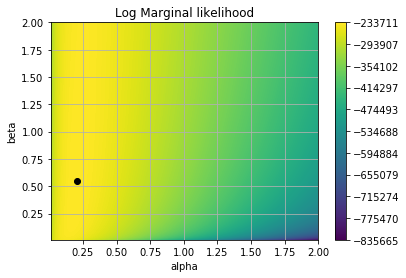
\includegraphics[width=7cm]{contour}}
	\caption{Marginal likelihood contour plot (as a function of the prior parameters, $\alpha$ and $\beta$). The circle on the left shows the optimum.}
	\label{fig:fig1}
	
	\fbox{ 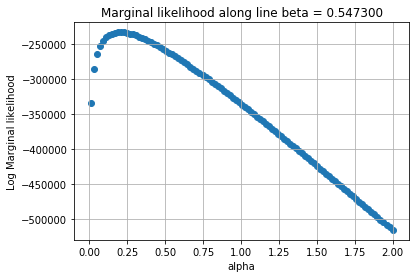
\includegraphics[width=7cm]{alpha}}
	\caption{Log marginal likelihood along the line of optimum $\beta$}
	\label{fig:fig1}
	
	\fbox{ 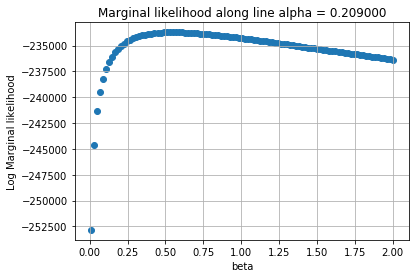
\includegraphics[width=7cm]{beta}}
	\caption{Log marginal likelihood along the line of optimum $\alpha$}
	\label{fig:fig1}
\end{figure}
Figure 1 shows the marginal likelihood as $\alpha$ and $\beta$ are varied in their respective ranges. The optimum value is $\alpha = 0.209$ and $\beta = 0.547$, close to our prescribed values of $\alpha = 0.2$ and $\beta = 0.5$ that were used to generate the data $\boldsymbol{y}$.

\section{Application to the Mechanics of Thin Shell Structures}

In this section we demonstrate the application of the proposed methodology to the deflection of thin shell structures. Thin shells are curved solids with one dimension significantly smaller than the other two. They are prevalent in nature, e.g., as insect wings or biological membranes and in engineering, most prominently in aerospace and automotive. Carefully designed curved thin shells have a load carrying capacity which is usually significantly higher than comparable flat structures.\\

\subsection{Problem Description}
We consider the composite beam shown in Figure 1 consisting of a gyroid core and two face plates. The gyroid is a triply periodic minimal surface with zero mean curvature and has recently been extensively explored in additive manufacturing applications, see e.g. Hussein et al. (2013); Abueidda et al. (2017). As known, cellular solids like the gyroid core can have mechanical properties that are orders of magnitude different from their constituent materials (Fleck et al., 2010). The length of the beam is 0.243m, its height, i.e. distance between the top and bottom plates, is 0.031m and its width is 0.031m. The gyroid core is described by the algebraic function\\

\begin{equation}
sin(\lambda x) cos(\lambda y) - sin(\lambda y) cos(\lambda z) - sin(\lambda y) cos(\lambda x) = 0
\end{equation}
with $\lambda = 20\pi$. The core and the two plates are modelled as thin shells and have a thickness of $t =$ 0.906 mm.
The beam is simply supported at a distance 11mm away from the boundaries (giving a span of 220mm). The Young’s modulus and the Poisson’s ratio are $E = 2.30 GPa$ and $\nu = 0.36$. The top plate is subjected to a line load of total distributed force $W$ acting in the negative z direction at mid span.
\subsection{Euler- Bernoulli Model}
The gyroid structure’s deflections can be estimated by an Euler-Bernoulli beam model, assuming that bending moment is proportional to curvature. To estimate the stiffness of our beam we need to know its Youngs modulus, which from lab tests was taken to be 2.30GPa, and the second moment of area. The second moment of area changes as the cross section of the beam changes. It can be crudely approximated by smearing all the material between the flanges into a central web, so that it looks like an I beam. The second moment of area was taken to be 19,560mm$^4$.

\subsection{Finite Element Model}
This model of the beam was compared to a thin-shell FEM model. The young’s Modulus of the material was taken to be $E = 2.30GPa$, the Poisson ratio as $\nu = 0.36$, and the boundary conditions as shown in the figure below **INSERT GRAPHIC OF BOUNDARY CONDITIONS - GE YIN WILL SEND THIS SOON**

\subsection{Obtaining the observed data}
The gyroid beam is a complex geometry that can only be manufactured via additive methods, such as 3D printing. The gyroid beam was 3D printed using the facilities in the Dyson Centre for Engineering Design and tested using the Instron machines at the Fatigue Lab at Cambridge University Engineering Department.

A laser system and reflective tape were used to measure the deflection of the beam across the span. The laser system measured the distance between two reflective tapes, once attached to the beam, and one attached to the intron machine, as pictured. The distances were subtracted from initial distances to get a deflection measurement, which was taken multiple times and averaged.
\begin{figure}[H]
	\centering
	\fbox{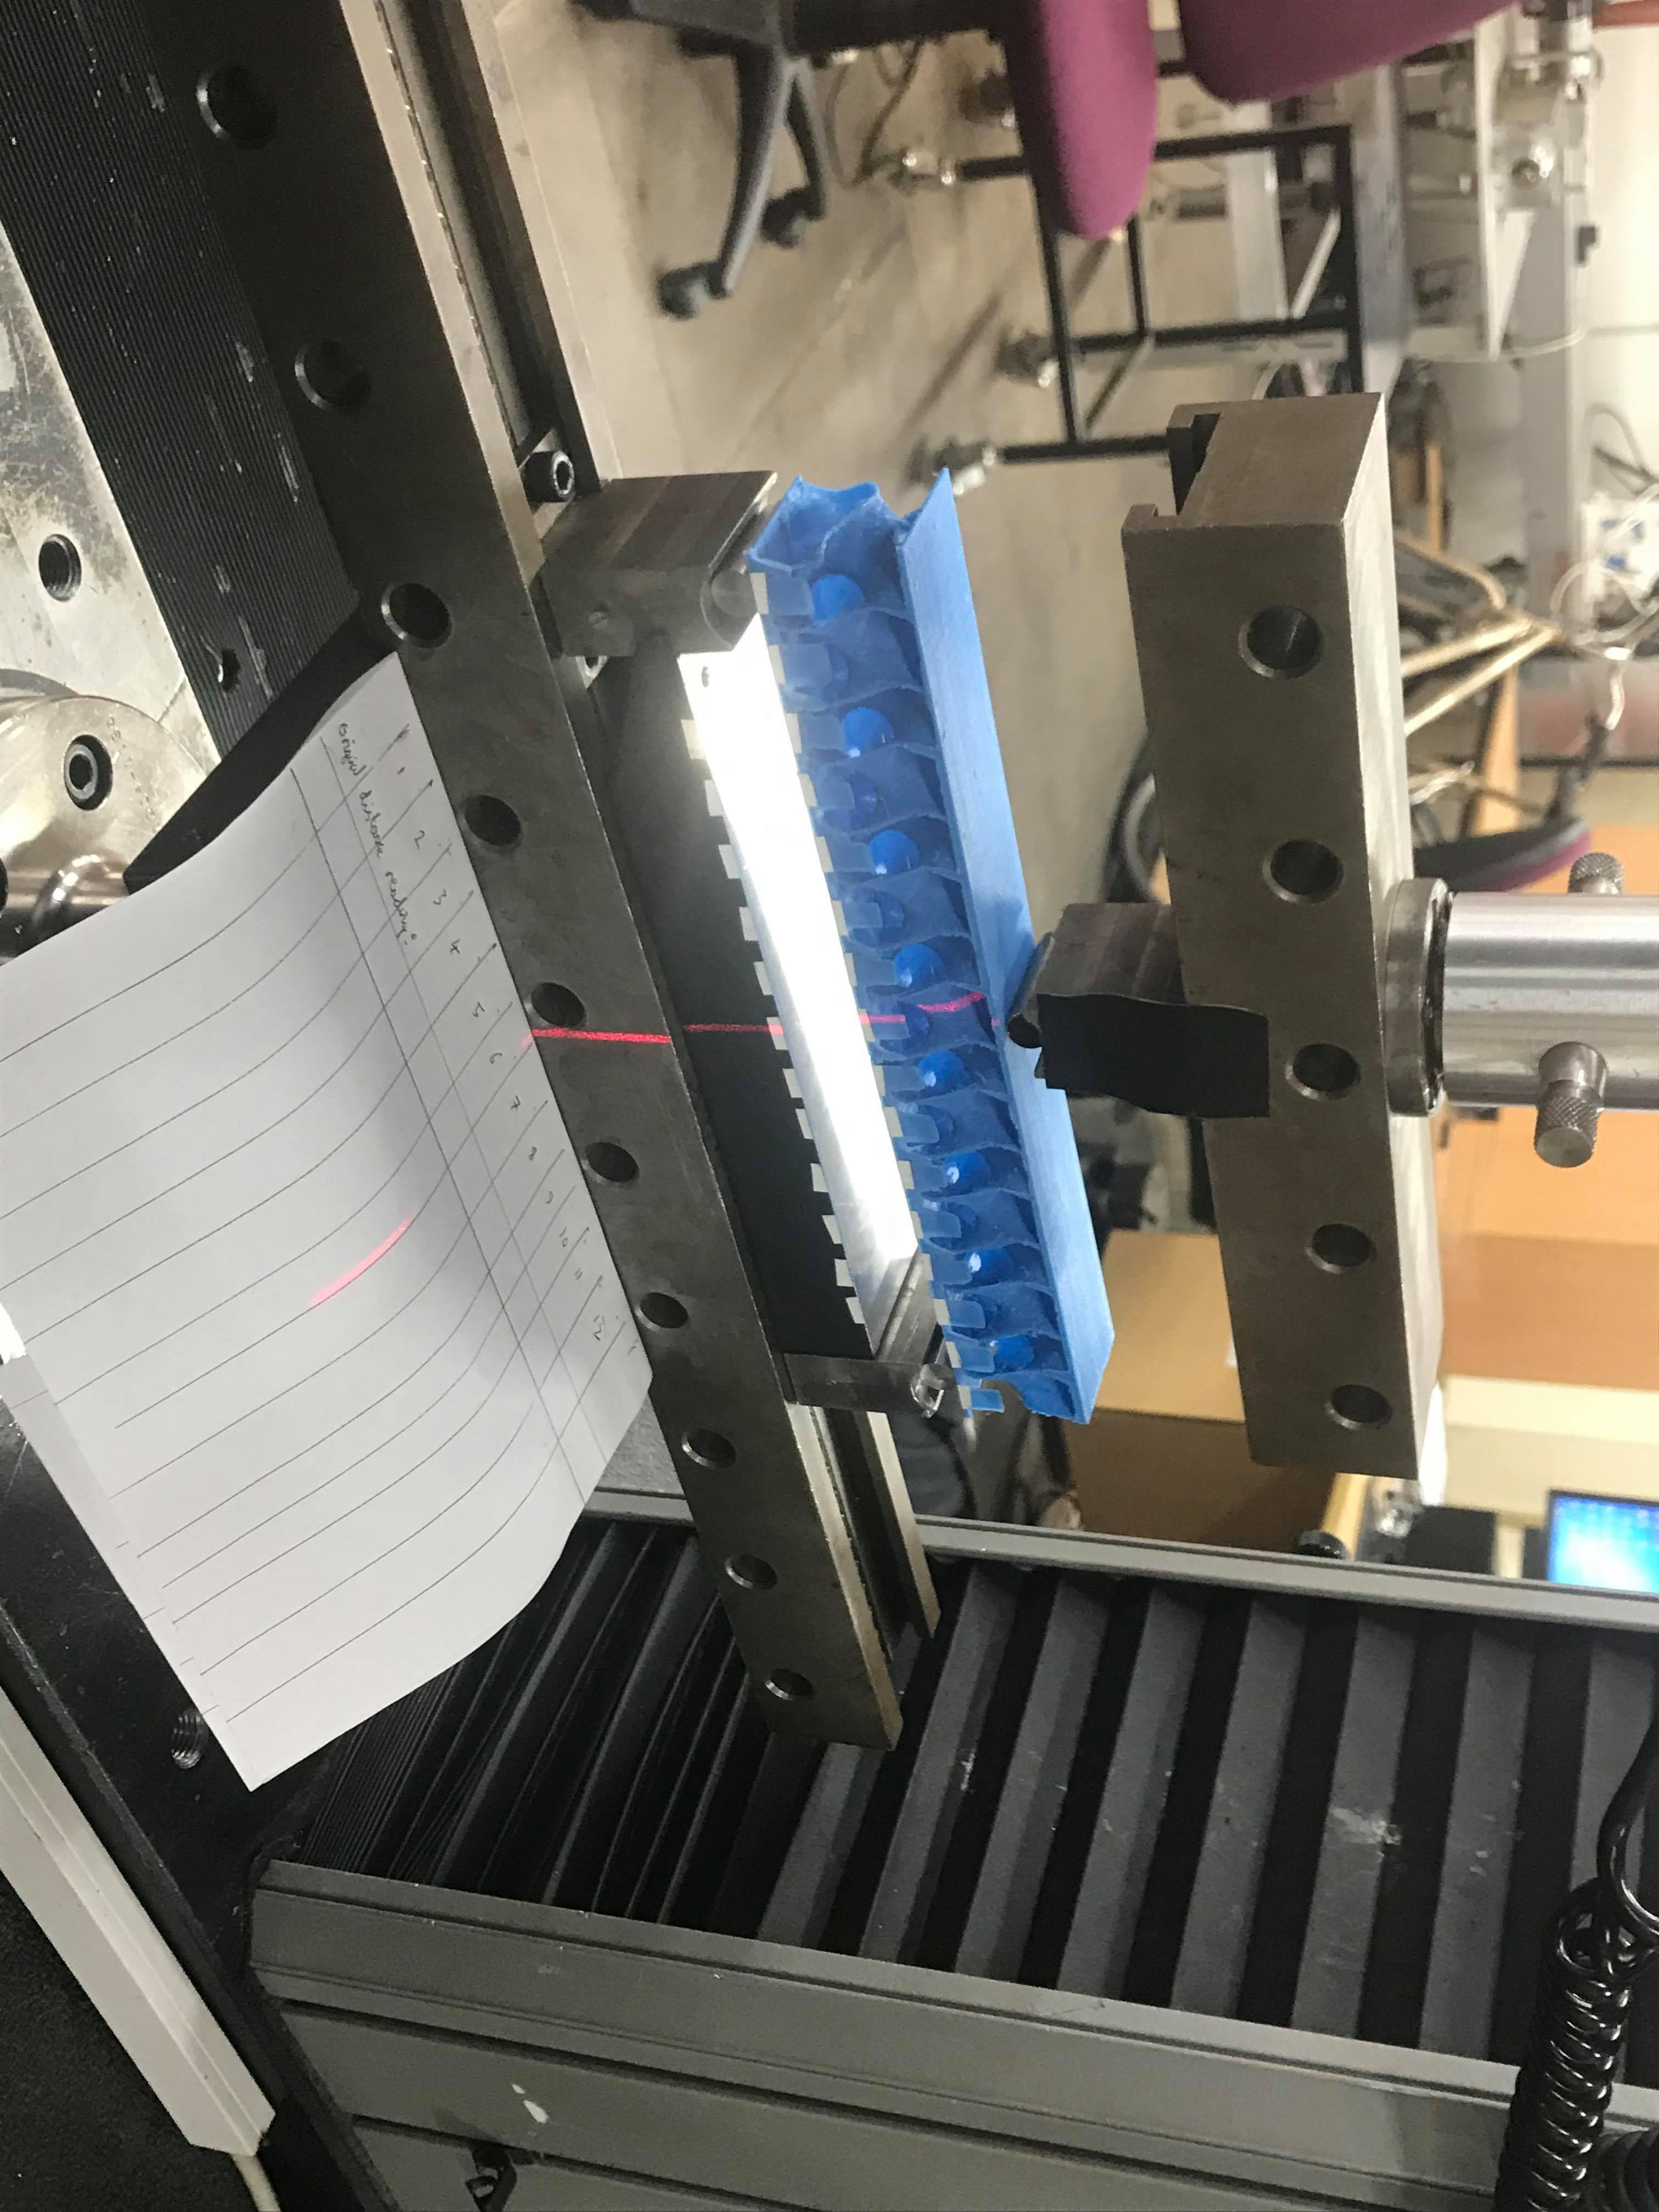
\includegraphics[trim={25cm 25cm 10cm 10cm},clip, angle=90,origin=c, width=15cm]{rotated}}
	\caption{Performing a 3-point bend test on the gyroid beam using an Instron machine. The laser measures the distance between the reflective tape placed on the bottom of the beam and the Instron machine. Some uncertainty in the measurement was introduced by rotating the laser round to take readings across the beam.}
\end{figure}
The laser was swung round on a tripod to point it at each set of tapes. This introduced some error in the deflection measurements as the act of rotating the laser on the tripod may have moved the tripod slightly in the direction of deflection.
The deflections were measured at loads of 200N, 250N and 300N.
A plot of the deflections at the different loads can be shown below. The 200N data can be seen to be quite noisy. This can be explained by the fact that the relative magnitude of the noise versus deflection is higher at lower deflections, and the noise had lowered for the 250N as we had taken more care with the measurements as we got used to the apparatus. It should be noted that the 300N load caused a small amount of plastic deformation, as deflection was outside of the linear-elastic regime.
\begin{figure}[H]
	\centering
	\fbox{ 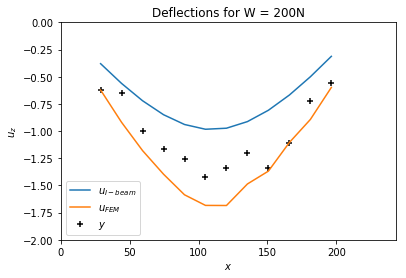
\includegraphics[width=9.8cm]{200N}}
	\caption{Deflection plot for the gyroid beam at W=200N. The orange line is the FEM model, the blue line is the Euler-Bernoulli model and the black crosses are the data from the instron test.}
	
	\fbox{ 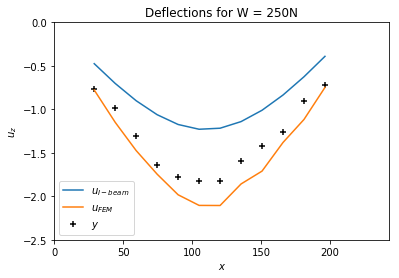
\includegraphics[width=9.8cm]{250N}}
	\caption{Deflection plot for the gyroid beam at W=250N.}
	
	\fbox{ 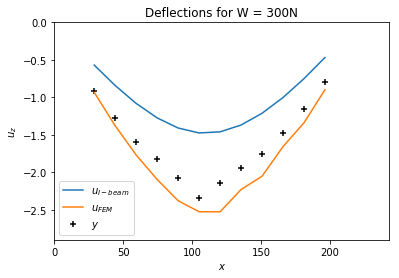
\includegraphics[width=9.8cm]{300N}}
	\caption{Deflection plot for the gyroid beam at W=300N.}
\end{figure}

\subsection{Comparing the Euler-Bernoulli Model to the Finite Element Model}

Looking qualitatively at the deflection results of figures 5-7, it can be seen that the FEM model tends to over-estimate the deflection, although it does pick up the general shape of the deflection fairly well. The Euler-Bernoulli beam model, on the other hand, tends to under-estimate the deflection. This can be explained by the plane section remains plane assumption of the Euler-Bernoulli model. This does not allow for shear deflections which are not be negligible since the beam is not thin, on the contrary: the depth is fairly large when compared to its length, with a depth/span ratio of 7.1. Furthermore, the bending stiffness of the beam may have been overestimated by smearing all of the material between the flanges onto a central web to calculate the second moment of area. By doing this, the web accounts for about a third of the beam's stiffness in the model.\\

Given this mismatch between the model and the data, it means that the error $\varepsilon_n = y_n - u_n$ is not independent, identically distributed, and so the statistical model cannot explain the data. In turn this means that the model has low FEM model and the marginal likelihood will not converge on a value of $\alpha$ and as shown in Figure 8 for the Euler Bernoulli model and Figure 9 for the FEM model.
\begin{figure}[H]%
	\centering
	\subfloat[Marginal likelihood contour plot as a function of the prior parameters, $\alpha$ and $\beta$]{\fbox{{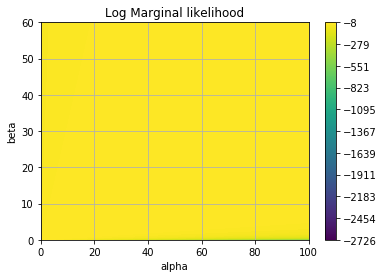
\includegraphics[width=7.5cm]{contour250I} }}}%
	\qquad
	\subfloat[Log marginal likelihood along the line of optimum $\beta$]{\fbox{{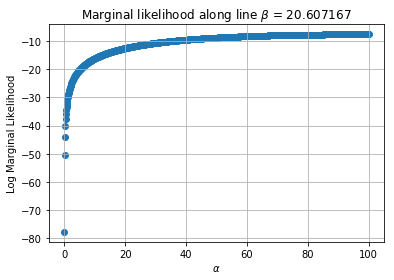
\includegraphics[width=7.5cm]{alpha250I} }}}%
	\qquad
	\subfloat[Log marginal likelihood along the line of optimum $\alpha$]{\fbox{{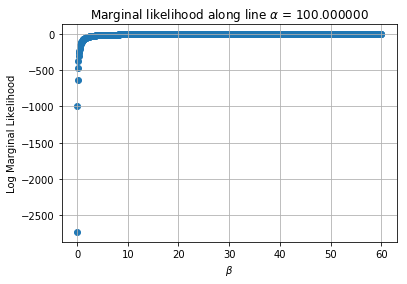
\includegraphics[width=7.5cm]{beta250I} }}}%
	\caption{Marginal likelihood plots showing the likelihood of the data given the Euler-Bernoulli beam model and parameters $\alpha$ and $\beta$}%
	\label{fig:example}%
\end{figure}

\begin{figure}[H]%
	\centering
	\subfloat[Marginal likelihood contour plot as a function of the prior parameters, $\alpha$ and $\beta$]{\fbox{{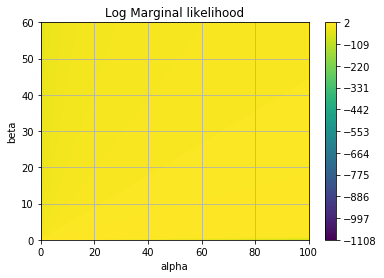
\includegraphics[width=7.5cm]{contour250FEM} }}}%
	\qquad
	\subfloat[Log marginal likelihood along the line of optimum $\beta$]{\fbox{{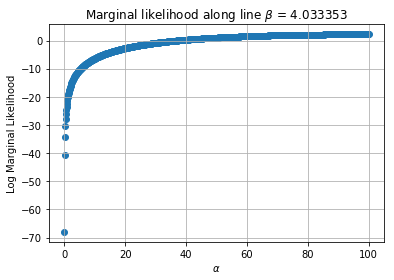
\includegraphics[width=7.5cm]{alpha250FEM} }}}%
	\qquad
	\subfloat[Log marginal likelihood along the line of optimum $\alpha$]{\fbox{{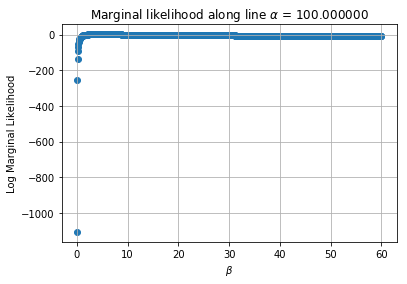
\includegraphics[width=7.5cm]{beta250FEM} }}}%
	\caption{Marginal likelihood plots showing the likelihood of the data given the FEM model and parameters $\alpha$ and $\beta$}%
	\label{fig:example}%
\end{figure}
The maximum likelihood was found at the edge of the search at $\alpha = 100$, and continues to rise for values $\alpha > 100$. It would be incorrect to select an arbitrary value of $\alpha$ and $\beta$ to compare the likelihood of each model, so we shall put a uniform prior distribution on the parameters $\alpha$ and $\beta$

\begin{equation}
\pi(\alpha, \beta|\kappa) = \kappa = \frac{1}{(\alpha_{max}- \alpha_{min})(\beta_{max}-\beta_{min})} \qquad \qquad \alpha_{min} < \alpha < \alpha_{max}, \beta_{min} < \alpha < \alpha_{max}
\end{equation}

to obtain the marginal likelihood

\begin{equation}
\begin{split}
P(\boldsymbol{y}|\boldsymbol{u}) & =\int{\int{P(\boldsymbol{y}|\boldsymbol{u},\alpha,\beta)\pi(\alpha,\beta| \kappa)}d\alpha} d\beta\\
\end{split}
\end{equation}

Since we have sampled $\alpha$ and $\beta$ over a discrete grid, then this integral can be approximated by

\begin{equation}
P(\boldsymbol{y}|\boldsymbol{u}) \approx\frac{1}{N}\sum_{i,j}{P(\boldsymbol{y}|\boldsymbol{u},\alpha_i,\beta_j)}
\end{equation}

where N is the number of samples in the grid.
The results of this value for the 2 models and 3 sets of data is shown in Table 1
\begin{table}[H]
	\centering
	\begin{tabular}{llr}  
		\toprule
		$\boldsymbol{y}$& FEM & Euler-Bernoulli Model \\
		\midrule
		$\boldsymbol{y}_{W = 200N}$ & 0.1718 & 0.0022\\
		$\boldsymbol{y}_{W = 250N}$ & 0.3749& 0.0001\\
		$\boldsymbol{y}_{W = 300N}$ & 0.0912& 0.0000\\
		\bottomrule
	\end{tabular}
\caption{$P(\boldsymbol{y}|\boldsymbol{u})$ values for each model and data set}
\end{table}

If we assume a uniform prior for each model $p(\boldsymbol{u_i})$, then the posterior for each model is simply:

\begin{equation}
P(\boldsymbol{u_i}|\boldsymbol{y}) = \frac{P(\boldsymbol{y}|\boldsymbol{u_i})}{\sum_j P(\boldsymbol{y}|\boldsymbol{u_j})}
\end{equation}

The ranking for each model is shown in Table 2 for the 2 models and 3 sets of data

\begin{table}[H]
	\centering
	\begin{tabular}{llr}  
		\toprule
		$\boldsymbol{y}$& FEM & Euler-Bernoulli Model \\
		\midrule
		$\boldsymbol{y}_{W = 200N}$ & 0.9874 & 0.0126\\
		$\boldsymbol{y}_{W = 250N}$ & 0.9997& 0.0003\\
		$\boldsymbol{y}_{W = 300N}$ & 0.9998& 0.0002\\
		\bottomrule
	\end{tabular}
	\caption{$P(\boldsymbol{u}|\boldsymbol{y})$ values for each model and data set}
\end{table}

It is shown that this method has overwhelmingly ranked the FEM model as the better model for all 3 data sets. As the loading, $W$, increased, the error between the data and the Euler-Bernoulli model increased more than the error between the data and the FEM model. This is reflected in table 2, as the posterior of the FEM model increases as the loading is increased, and the posterior for the Euler-Bernoulli model decreases as the loading is increased.

\section{Conclusion}
It was shown that the FEM model was better than the Euler-Bernoulli model at predicting the data.\\
The statistical model used to explain the data had low FEM model, primarily because the assumption that the mean was known was unfounded. Further work could change the model to do a Bayesian analysis on the mean. However, for the purposes of ranking the two models, the method used seemed to work well, picking the FEM model as the clearly superior model at predicting the data.


\bibliographystyle{unsrt}  
%\bibliography{references}  %%% Remove comment to use the external .bib file (using bibtex).
%%% and comment out the ``thebibliography'' section.

\begin{thebibliography}{0}
	
	\bibitem{stat}
	Girolami, M., Gregory, A. Yin, G., Cirak, F. (2019). The Statistical Finite Element Method
	
	\bibitem{Abueidda}
	Abueidda, D. W., Bakir, M., Abu Al-Rub, R. K., Bergstr\"{o}m, J. S., Sobh, N. A., and Jasiuk, I. (2017).
	Mechanical properties of 3d printed polymeric cellular materials with triply periodic minimal surface
	architectures. Materials %& Design, 122:255–267.
	
	\bibitem{Fleck}
	Fleck, N. A., Deshpande, V. S., and Ashby, M. F. (2010). Micro-architectured materials: past, present and
	future. Proceedings of the Royal Society of London A: Mathematical, Physical and Engineering Sciences,
	466:2495–2516.
	
	\bibitem{Hussein}
	Hussein, A., Hao, L., Yan, C., Everson, R., and Young, P. (2013). Advanced lattice support structures for
	metal additive manufacturing. Journal of Materials Processing Technology, 213:1019–1026.
	
	\bibitem{Jordan} 
	"The Conjugate Prior for the Normal Distribution" Michael I. Jordan (2010). The Conjugate Prior for the Normal Distribution. Stat260: Bayesian Modelling and Inference, University of California, which can be viewed at https://people.eecs.berkeley.edu/~jordan/courses/260-spring10/lectures/lecture5.pdf (accessed July 2019).
	

\end{thebibliography}


\end{document}
